\section{Implementation plan}\label{sec:plan}

\subsection{Technology choices}

\begin{center}
\small
\begin{tabularx}{\linewidth}{@{}L{3.4cm}L{4.2cm}Y@{}}
\toprule
\textbf{Component} & \textbf{Technology} & \textbf{Reason}\\
\midrule
Admission proxy, KYA runner, egress gateway & Go & Same language as AX; reuses its generated gRPC types and runner package; strong HTTP/TLS libraries.\\
Passport authority & Go, PostgreSQL & Ed25519 and JWS in the standard ecosystem; small, auditable service.\\
Verifier SDK & Java (Spring Boot starter), Go middleware & Covers the most common backend stacks; the team already knows Spring Boot.\\
Trust observer & Python (FastAPI, scikit-learn), Redis Streams or NATS & Fast iteration on features and models; isolation forest in scikit-learn.\\
Audit ledger & PostgreSQL & Append-only table plus hash chain; simple to operate.\\
Console & React + TypeScript & Standard web front end.\\
Demo relying parties & Spring Boot (shop), Go (payments) & Realistic targets for the evaluation.\\
Deployment & Kubernetes manifests / Helm, GitHub Actions & Reproducible installation next to AX.\\
\bottomrule
\end{tabularx}
\end{center}

\subsection{Repository layout}

\begin{lstlisting}[language={}]
agentpassport/
  cmd/
    kya/                 # CLI helper: login, policy apply, passport inspect
    admission-proxy/
    passport-authority/
    egress-gateway/
    kya-runner/          # embeds github.com/google/ax/runner
  pkg/
    passport/            # claims, signing, verification (shared)
    httpsig/             # RFC 9421 profile
    policy/              # AgentPolicy parsing and visa intersection
  sdk/
    java/kya-spring-boot-starter/
    go/kyaverify/
  observer/              # Python service + models
  console/               # React app
  demo/
    shop/                # Spring Boot relying party
    payments/            # Go relying party
    agents/              # scripted and LLM-driven demo agents
  attacks/               # attack-suite scenarios and runner
  deploy/                # Helm charts, AX/Substrate install notes
  docs/
\end{lstlisting}

\subsection{Work packages}

\begin{center}
\small
\begin{tabularx}{\linewidth}{@{}lL{4.4cm}Y@{}}
\toprule
\textbf{WP} & \textbf{Title} & \textbf{Outputs}\\
\midrule
WP0 & Platform setup & AX + Agent Substrate running on a cluster; pinned AX commit; egress-control experiment (Section~\ref{sec:seams}).\\
WP1 & Specification & Passport format, signature profile, policy schema, threat model (this document, refined).\\
WP2 & Identity core & Passport authority, admission proxy, \code{kya} CLI, OIDC integration.\\
WP3 & Enforcement & KYA runner, egress gateway (allowlist, TLS, signing, metering).\\
WP4 & Relying-party side & Verifier SDKs, step-up approvals, demo shop and payments API.\\
WP5 & Trust observer & Event pipeline, features, rules, anomaly model, AX suspension.\\
WP6 & Delegation and audit & Child passports, budget reservation, hash-chained ledger, checkpoints.\\
WP7 & Console & Agent, approval, incident and audit views.\\
WP8 & Evaluation & Attack suite, benchmarks, ablation study, final report.\\
\bottomrule
\end{tabularx}
\end{center}

\subsection{Timeline}

The project spans two semesters (Figure~\ref{fig:timeline}). The first semester delivers a working vertical slice: a task launched through the admission proxy, with a passport, whose requests are signed by the gateway and verified by the demo shop. The second semester adds the observer, delegation, the console and the full evaluation.

\begin{figure}[H]
  \centering
  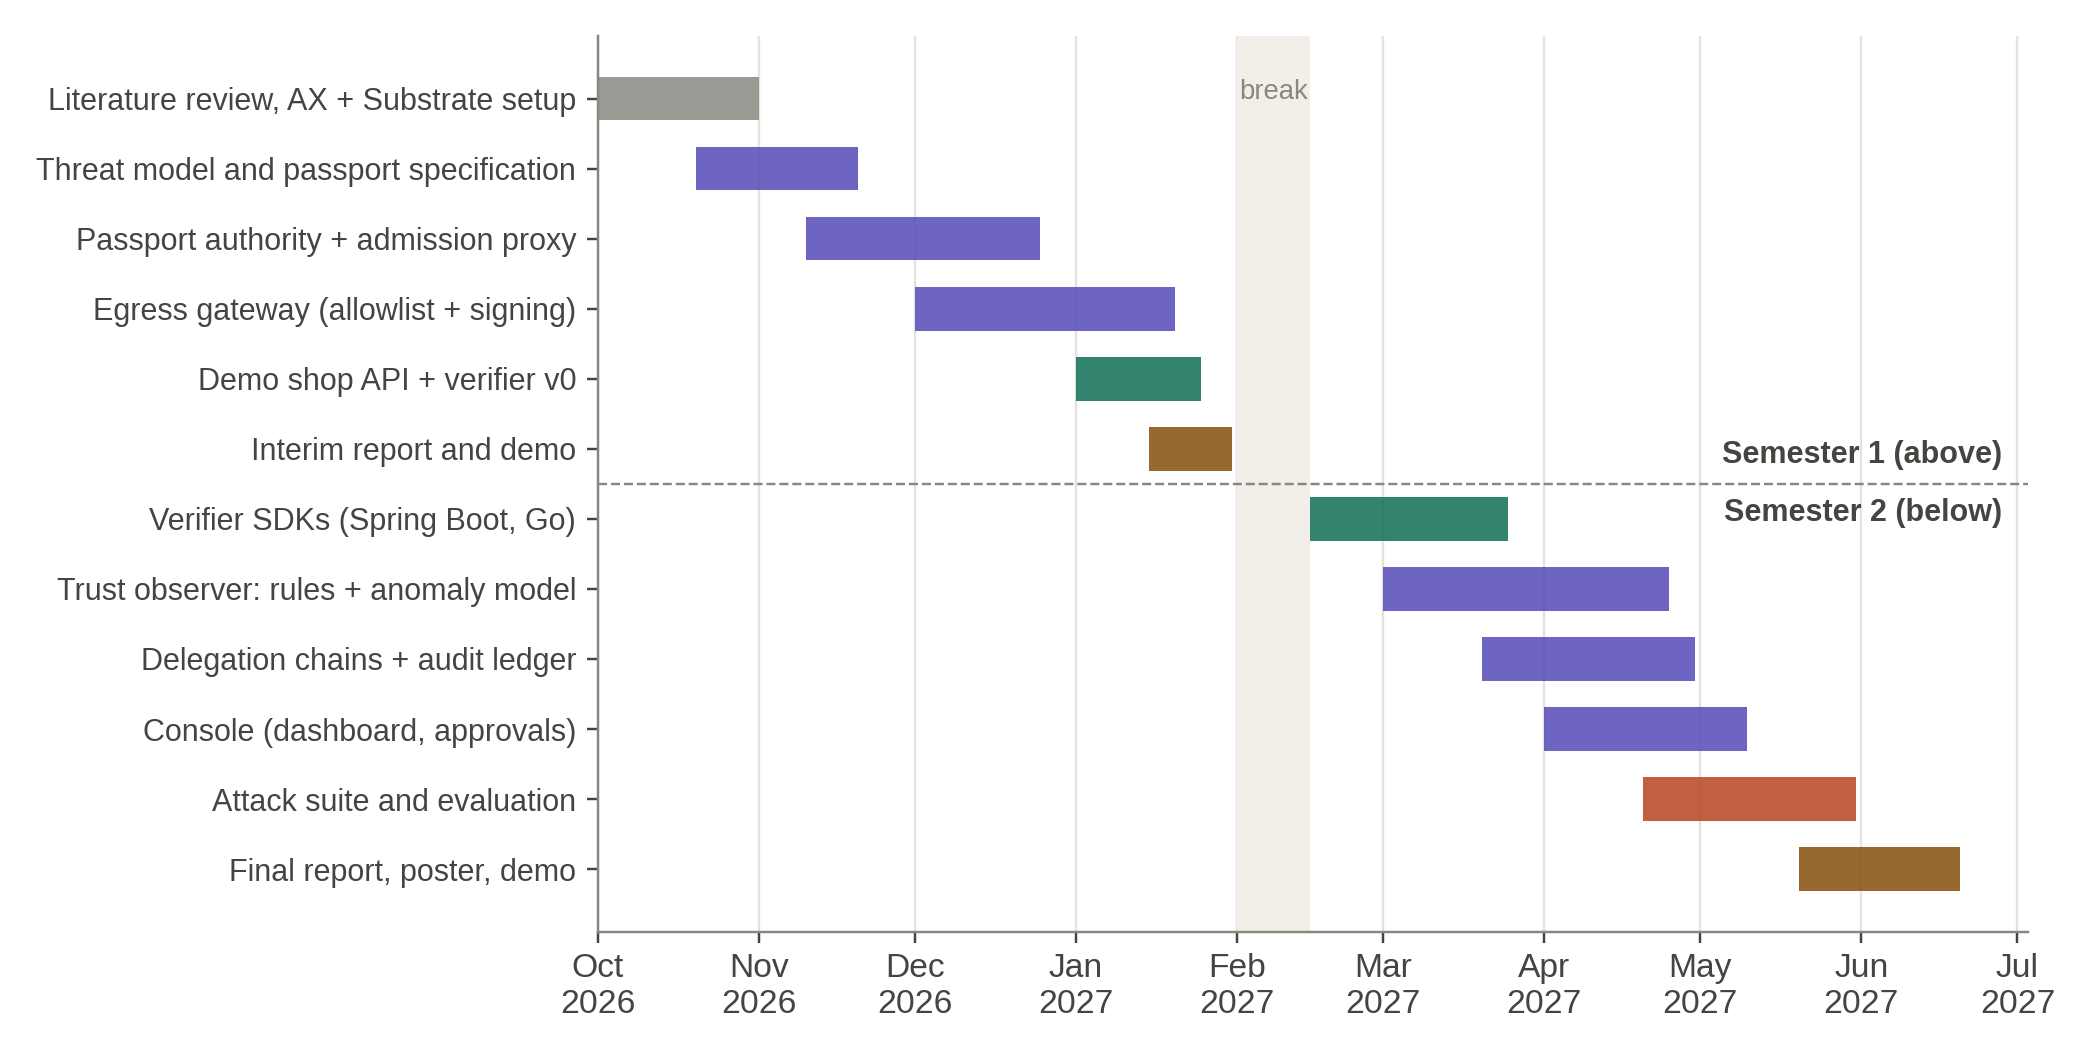
\includegraphics[width=\linewidth]{timeline.png}
  \caption{Planned timeline. Colours follow the diagrams: purple for KYA core components, green for relying-party work, red for evaluation, brown for reports.}
  \label{fig:timeline}
\end{figure}

\textbf{Milestones.}
\begin{itemize}
  \item \textbf{M1 (end of November 2026):} AX running; passport spec frozen; first passport issued for a real AX task.
  \item \textbf{M2 (end of January 2027):} vertical slice demo, i.e.\ Example~1 and the gateway half of Example~2 working end to end; interim report.
  \item \textbf{M3 (end of April 2027):} observer suspends tasks automatically; delegation works; Examples~2--6 reproducible.
  \item \textbf{M4 (June 2027):} evaluation complete; final report, poster and live demonstration.
\end{itemize}

\subsection{Team organisation}

Work packages are grouped into roles so that each team member owns a coherent part while everyone contributes to the evaluation. Final assignment will be made at the kick-off meeting.

\begin{center}
\small
\begin{tabularx}{\linewidth}{@{}L{3.6cm}L{3.2cm}Y@{}}
\toprule
\textbf{Role} & \textbf{Main WPs} & \textbf{Focus}\\
\midrule
Platform and infrastructure & WP0, WP3 & Cluster, AX, runner, gateway, deployment.\\
Identity and cryptography & WP1, WP2, WP6 & Passport authority, signatures, delegation, ledger.\\
Relying party and SDK & WP4, WP7 & Verifier SDKs, demo services, console.\\
Observer and evaluation & WP5, WP8 & Features, anomaly model, attack suite, benchmarks.\\
\bottomrule
\end{tabularx}
\end{center}

\subsection{Risks}

\begin{center}
\small
\begin{tabularx}{\linewidth}{@{}L{4.2cm}L{1.4cm}Y@{}}
\toprule
\textbf{Risk} & \textbf{Impact} & \textbf{Mitigation}\\
\midrule
AX introduces breaking API changes (it is \code{v1alpha1}). & High & Pin one AX commit for the whole project; keep all AX-specific code in thin adapters (proxy forwarding, runner embedding, suspend client).\\
Agent Substrate is hard to install or needs more resources than available. & High & Start with WP0 immediately; request cloud education credits; as a last resort, implement a minimal ``fake AX'' with the same gRPC API on plain Kubernetes pods so that the KYA layer can still be developed and evaluated.\\
Sandbox egress cannot be restricted to the gateway. & Medium & Use Kubernetes NetworkPolicy on worker pods; otherwise fall back to proxy variables and state the limitation clearly.\\
TLS interception breaks some agent libraries (certificate pinning). & Medium & Offer the explicit-proxy mode; document affected libraries.\\
Anomaly model has too many false positives. & Medium & Rules first, model second; conservative thresholds; suspension instead of deletion.\\
Scope creep (KYA is a broad topic). & Medium & Milestones define a minimum viable system; stretch goals (credential injection, Biscuit, hardware keys) are explicitly optional.\\
\bottomrule
\end{tabularx}
\end{center}

\subsection{Deliverables}

\begin{enumerate}
  \item Open-source code for all components, with Helm charts to install AgentPassport next to AX.
  \item The \textbf{AgentPassport specification}: passport claims, signature profile and policy schema, written so that others can implement compatible verifiers.
  \item Verifier SDKs for Spring Boot and Go, published as packages.
  \item The attack suite and benchmark scripts, reproducible by others.
  \item Interim and final reports, a poster, and a recorded end-to-end demonstration of Examples~1--6.
\end{enumerate}
